\documentclass[letterpaper,12pt]{exam}

\RequirePackage{GE05}
% this inputs graphicx, too
\RequirePackage{comment}
\RequirePackage[hypertex]{hyperref}
    \hypersetup{colorlinks=true,urlcolor=blue,linkcolor=red}

\newcommand{\NX}{\mbox{\em NX\/}}
\newcommand{\POP}{\mbox{\em POP\/}}

\def\ClassName{The Global Economy}
\def\Category{Professor David Backus}
\def\HeadName{Group Project \#4}

\printanswers 

\begin{document}
\parindent = 0.0in
\parskip = \bigskipamount
\thispagestyle{empty}%
\Head

\centerline{\large \bf \HeadName:  Labor and Trade}%
\centerline{Revised:  \today}

\medskip
{\it Submit via Blackboard by 9am March 2.}

\begin{questions}

% ----------------------------------------------------------------------
\question {\it Labor market practice.\/}  
Your first day on the job at General Electric, 
you are given 4 hours to collect the information for 
a 5-minute presentation to your group summarizing the 
labor market issues a manufacturer would face in 
Brazil, Poland, and Singapore.    
Once you get over your initial panic, 
you contact your Global Economy professor, who suggests you look at
the Global Economy resource page, including     
%
\begin{itemize}

\item The Bureau of Labor Statistics'
\href{http://www.bls.gov/fls/hcaesupptabtoc.htm}
{Foreign Labor Statistics};


\item The World Bank's
\href{http://www.doingbusiness.org/}
{Doing Business};   

\item The Economist Intelligence Unit's various 
\href{http://db.eiu.com/topic_view.asp?pubcode=CP&title=Country+Profile}{reports} 
and 
\href{http://www.countrydata.bvdep.com/cgi/template.dll?product=101&user=ipaddress}
{databases}.  

\end{itemize}
%
You quickly turn this information into a series of charts 
and bullet points 
that highlight the salient differences among these countries.  (50~points) 

\begin{solution}
Here's a quick sketch of the kind of data you
might collect, with the US included for comparison: 
% 
\begin{center}
\begin{tabular}{lccccc}
\hline\hline
Indicator   & Brazil & Poland & Singapore  &  US \\
\hline\hline 
Hourly total comp (USD) & 4.91 & 4.99   & 8.55  &  23.82  \\
Employment rigidity (index)    & 46   & 37   &  4  &  0  \\
Firing costs (weeks of pay) &  37   &  13   &  0  & 0  \\
Education of adults (yrs) &  4.9  &  9.8  & 7.0  &  12 \\
\hline\hline 
\end{tabular}
\end{center}
Sources:  BLS, Doing Business, and NationMaster.com.  
Most recent year available.   

What do we make of this?  
Labor is cheap in all of these countries relative to the US.  
Education is lowest in Brazil.
Labor markets are most flexible in Singapore. 
In a real report, you'd want to flesh out what these factors mean
to GE:  how these factors and related ones would affect their
business.  
Does education matter?  Flexibility?  

\end{solution}

% ----------------------------------------------------------------------
\question {\it Mexico and NAFTA.\/} 
Like many developing countries, 
Mexico followed a policy of ``import substitution'' after World War II, 
using high tariffs to help local industry ``substitute'' 
local products for imports.  
Trade policy changed dramatically in 1994,
when Mexico signed the North American Free Trade Agreement (NAFTA)
with Canada and the United States.
Under NAFTA, tariffs between these countries fell on a wide range 
of products and the volume of trade expanded rapidly.  
The question is how the change in policy affected overall 
economic performance.  

Looking at Figure \ref{tab:mexico}, you decide to look at two periods, 
1950-80 and 1994-2003, throwing out the lost decade of the 1980s 
(a story for another time).  
In the first period, tariffs were high, in the second, much lower.  
Using the data provided and your own analytical skills, you decide to 
examine the impact of trade policy and the performance 
of Mexico's economy.  

\begin{figure}[!]
    \centering
    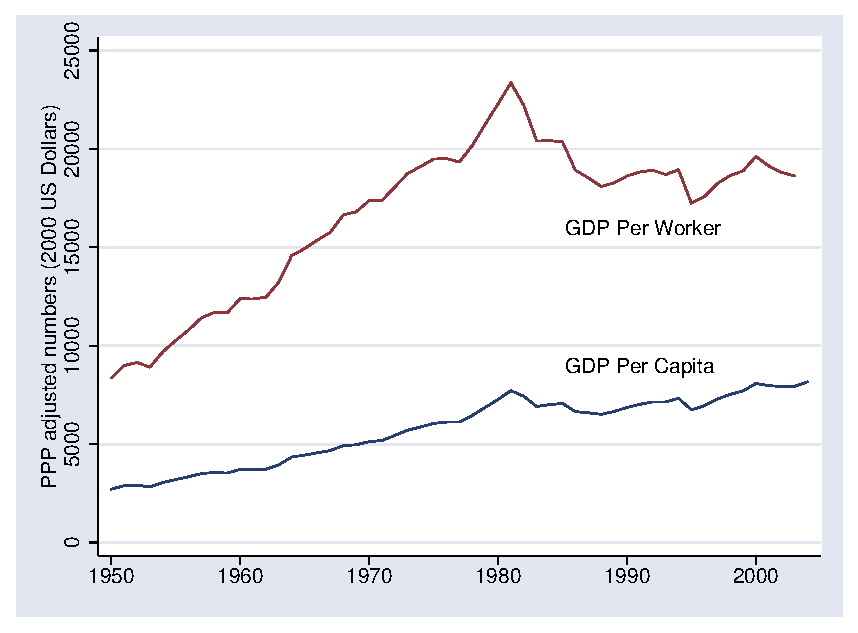
\includegraphics[scale=0.8]{pwtmexypopyl.eps}
    \caption{GDP Per Capita and GDP Per Worker in Mexico.}
    \label{fig:mexico}
\end{figure}

\begin{table}[!]
    \centering 
    \tabcolsep = 0.2in
    \begin{tabular}{lccc}
    \hline\hline
    Year    &  $Y/\POP $  &  $Y/L$  &  $K/L$  \\
    \hline\hline
    1950 &  2,709 &  8,358   &  10,066 \\
    1980 &  7,271 &  23,360  &  48,334  \\
    1994 &  7,328 &  18,943  &  45,444 \\
    2003 &  7,938 &  18,628  &  47,089 \\
    \hline\hline
    \end{tabular}
    \caption{Output and Capital in Mexico.
    Data from the Penn World Tables.  Output (GDP) and capital
    are measured in 2000 US dollars.}
    \label{tab:mexico}    
\end{table}

\begin{parts}
\part How do growth in GDP per capita ($Y/\POP$) 
and GDP per worker ($Y/L$) differ between the two periods?  
What is the source of any differences between the two measures?    
(15~points)

\pagebreak % ****
\part What are the sources of growth in GDP per worker 
in the two periods?  
Note specifically growth in (total factor) productivity.  
(20~points)

\part How would you expect a reduction in trade barriers  
to affect productivity?
Is that what you see?  
Speculate on why or why not.   
(15~points)
\end{parts}

\begin{solution}
%
\begin{parts}

\part We compute continuously-compounded growth rates the usual way.
For GDP per capita, the growth rates 
are 3.29 (1950-80) and 0.89 (1994-2003).  
Both are expressed as percentages.
For GDP per worker, the growth rates are 3.43 and $-0.19$, respectively.  
With both measures, growth is much slower in the later period.  
The difference has to come from differences in the growth rates 
of population and workers; equivalently, the ratio of 
of workers to population must be changing.  
Evidently the relatively slow growth in GDP post 1994
is worse than it looks:  part of it is an increase 
in the fraction of the population working.  

%Grading:  8 points for computing the growth rates, 
%2 for understanding the difference between them.  

\part The usual growth accounting exercise.  
Our decomposition of the growth rate of output per worker is 
\[
        \gamma_{Y/L} \;=\; \gamma_A + \alpha \gamma_{K/L}  
\]
with $\alpha = 1/3$.
The letter $A$ stands for total factor productivity (TFP).    
For the two periods, we get 
\begin{eqnarray*}
    \mbox{1950-1980:} &&  3.43  \;=\; 1.68 \mbox{ (A)} 
                +  1.74 = 5.23/3 \mbox{ (K/L)}   \\
    \mbox{1994-2003:} &&  -0.19 \;=\; -0.32 \mbox{ (A)} 
                +  0.13 \mbox{ (K/L)} .
\end{eqnarray*}
There's apparently a drop in TFP growth ($\gamma_A$).  

%Grading: 20 points for getting the numbers exactly right, 
%partial credit for other answers.  

\part This is the issue:  we have seen that reducing trade barriers
is like increasing TFP.  
But here we see that TFP fell during the period when trade 
barriers were lowest and trade was highest.  
What went wrong?  
One possibility is that the theory of trade is wrong:  
trade doesn't increase productivity.
Another is that it takes time for the reallocation 
suggested by trade to take place.  
Yet another is that something else is going on:  
the crisis in 1994-95 evident in the figure, 
some problem that inhibits the reallocation 
called for by trade, 
or anything else that crosses your mind.  
My own list would include:
frictions in labor and capital markets (it's relatively 
difficult for small firms to borrow money)
and restrictions on entry (in some industries, 
business leaders use government connections 
to discourage competition). 
Whether this is enough to explain what we see is hard to say.  

%Grading: 7 points for noting the presumed connection 
%between trade and productivity and disparity with the evidence, 
%3 for any reasonable discussion of what might be going on.  

\end{parts}
\end{solution}

\end{questions}

\vfill \centerline{\it \copyright \ \number\year \ NYU Stern
School of Business}

\end{document}

\question {\it Labor market theory.\/} As background to a
consulting assignment, you have been asked to work through an
example to illustrate the impact of
minimum wage legislation and payroll taxes on employment and
unemployment. You decide to adapt the framework of your 
{Global Economy} class notes, 
working through the demand for labor
of a single firm producing widgets according to the production
function $Y= A K^{1/3}L^{2/3}$. For simplicity, you assume that
$A=K=1$ and that the price of widgets is 1, too.  The supply of
labor rises with the wage $w$: $L^{s}=w^{2}$.
% ?? *** make this w^3 to match up exponents 
%
\begin{enumerate}

\item Describe, first, how the labor market might work in this
economy if there were no labor market restrictions.  
What is the wage?
Employment? Unemployment?  (10~points)

\item Now consider the effect of introducing a minimum wage $w_{m}$.  
What are the employment and unemployment rates if $w_{m}=1$?
If $w_{m}=0.5$?  
%How does this market differ from the one above?
If $w_m = 1$, describe qualitatively how much 
an unemployed person be willing to pay a recruiter
to find a job.  
(10~points)

\item Suppose workers differ in productivity, 
with some contributing effectively 1.5 units of labor 
per unit paid, and others contributing only 0.5 units.  
Describe qualitatively how  you would expect a minimum wage  
to affect the two types of workers.  
(10~points)

\end{enumerate}

%\begin{comment}
Answer. The firm's optimal level of labor (its labor demand) is
such that the gain of adding one more worker is equal to its cost.
The marginal gain is the derivative of sales with respect to
labor: $\frac{2}{3}pAK^{1/3}L^{-1/3}$. The marginal cost is simply
the wage $w$. Therefore, since $p=K=A=1$, the demand for labor is
\[
    L^{d} \;=\; \left(\frac{3}{2}w\right)^{-3}.
\] 

\begin{enumerate}
\item The equilibrium is reached when demand equals supply. That
is:
\[ 
    \left(\frac{3}{2}w\right)^{-3} \;=\; w^{2}.
\] 
Solving for $w$, we obtain that the equilibrium wage is
\[ 
    w^{*} \;=\; \left(\frac{3}{2}\right)^{-3/5}=.78.
\] 
The level of employment is
\[ 
    L^{*} \;=\; \left(\frac{3}{2}w^{*}\right)^{-3}={w^{*}}^{2}=.61.
\] 
The unemployment rate is $0$. Since there is no distortion, all
individuals that would like to work at the equilibrium wage rate
get a job.

\item If $w_{m}=1$, the demand for labor is
$L^{d}=\left(\frac{3}{2}\times 1\right)^{-3}=.30$. Instead the
supply is $L^{s}=1^{2}=1$. Therefore the level of employment is
$.30$. The unemployment rate is $\frac{1-.3}{1}=70\%$. Every
unemployed will be willing to pay a recruiter up to the difference
between the ongoing wage ($1$) and his/her reservation wage. The
reservation wage is different across unemployed, and can be read
off the labor supply curve.

%%%%%%%%%%%%%%%%%%%%%%%%%%%%%%%%%%%%%%%%%%%%%%%%%%%%%%%%%%%%%%%%%%%%%%%%%%%%

\begin{figure}[h]
\begin{center}
\begin{picture}(300,200)(-30,-20)%

\footnotesize%
\put(-30,0){\vector(1,0){300}}%
\put (0,-20){\vector(0,1){200}}%
\put(265,-14){$L$}%
\put(-15,175){$w$}%
\put (154,157){$L^{s}(w)$}%
\put(44,157){$L^{d}(w)$}%

% Demand Curve
\qbezier(45,145)(90,41)(165,10)%

% Supply Curve
\qbezier(45,25)(80,41)(175,140)%

\qbezier[60] (0,92)(65,92)(128,92)%
\qbezier[40] (71,0)(71,46)(71,93)%
\qbezier[40] (128,0)(128,46)(128,93)%

\qbezier[40] (0,62)(50,62)(95,62)%
\qbezier[30] (95,0)(95,31)(95,62)%

\put(-38,60){$w^{*}=.76$}%
\put(-33,90){$w_{m}=1$}%

\put(95,-18){$.61$}%

\put(65,-18){$.30$}%
\put(130,-18){$1$}%

\end{picture}
\end{center}
\caption{With and without unemployment.} \label{fig:minimum1}
\end{figure}

%%%%%%%%%%%%%%%%%%%%%%%%%%%%%%%%%%%%%%%%%%%%%%%%%%%%%%%%%%%%%%%%%%%%%%%%%%%%

The wage $w_{m}=.5$ is below the equilibrium rate. This means that
the minimum wage is not binding. The outcome in terms of wage and
employment is going to be the same as in part (a).

\item You might guess that the minimum wage would  affect 
the low-skilled workers more than the high-skilled. 
Why?  Because the high-skilled are worth more than the minimum 
wage, so they will be hired (presumably) something close to their 
productivity.
But if the productivity of the low-skilled is below the minimum wage, 
they won't be hired. 
The result is that the unemployed will consist predominantly 
(perhaps entirely in this setup) of the low-skilled. 

\end{enumerate}
%\end{comment}

